\chapter{Tuning the models}

\section{Inertial circles in the dynamic model}

When the dynamic model was tested, some trajectories traced out large spirals, behavior uncharacteristic of atmospheric flow.
Figure \ref{fig:boston_inertial} shows an example of one such trajectory.
The parcel's spiral is a result of the Coriolis force term in the dynamic equations.
In the Northern Hemisphere, the direction of the Coriolis force is to the right of a parcel's motion.
[[[Why are inertial circles observed in the ocean and not the atmosphere? What metric predicts this? Ekman number?]]]

The period $T$ and radius $R$ of an inertial circle are

\begin{align}
    T &= \frac{2 \pi}{f} \\
    R &= \frac{v}{f}
\end{align}

where $f$ is the Coriolis parameter.

[[[To do: show that period and radius of this trajectory are what you'd expect for an inertial circle.]]]

\begin{figure}
    \centering
    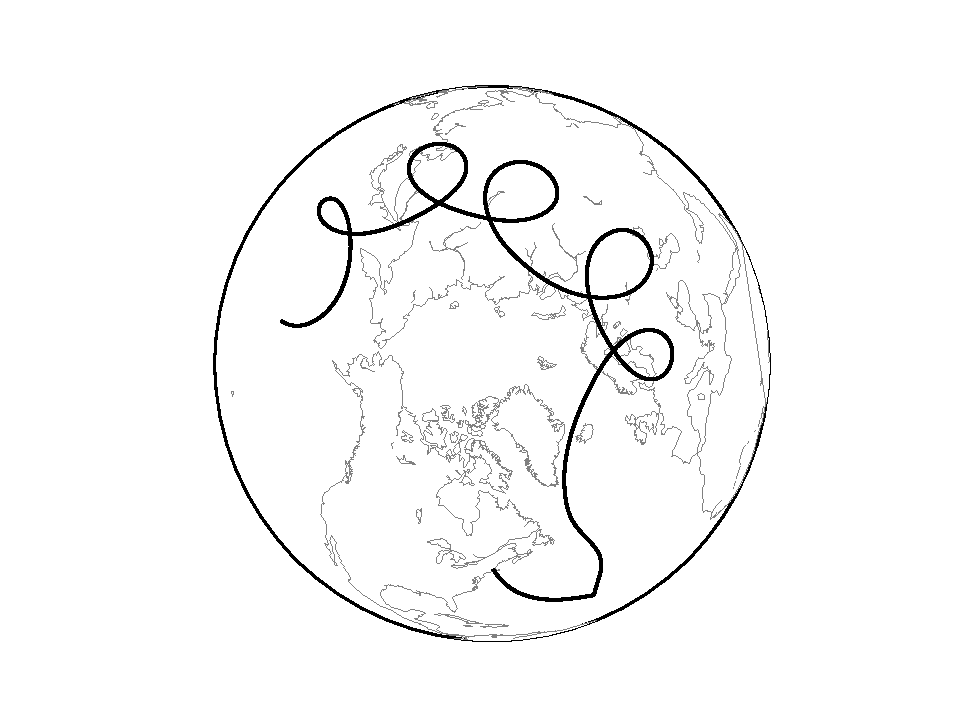
\includegraphics[width=\textwidth]{boston_inertial.pdf}
    \caption{A parcel launched from 41.75$^\circ$N, 71.25$^\circ$W. Five inertial circles are visible in the latter part of the trajectory.}
    \label{fig:boston_inertial}
\end{figure}

\begin{figure}
    \centering
        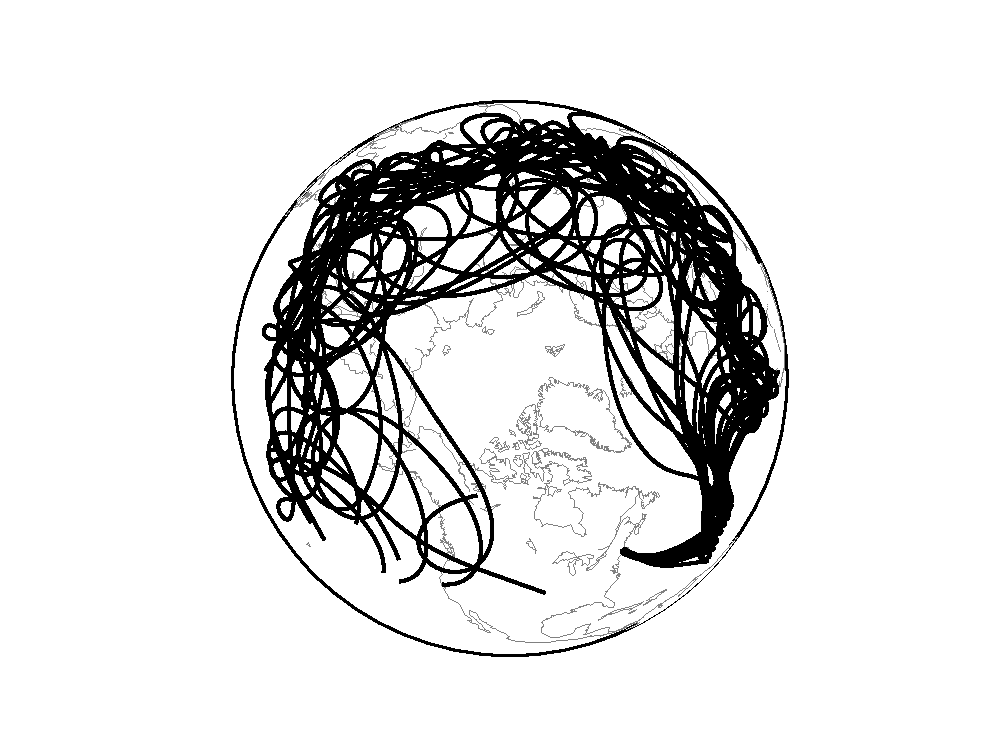
\includegraphics[trim=30 30 30 30, clip, width=0.49\textwidth]{force_180.eps}
        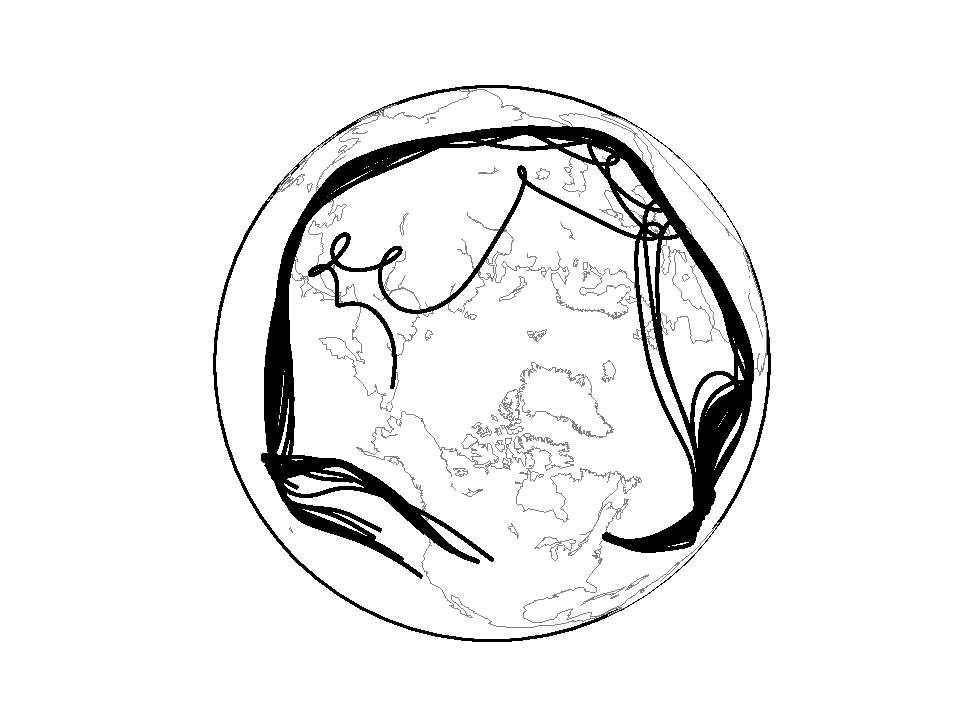
\includegraphics[trim=30 30 30 30, clip, width=0.49\textwidth]{friction_180.pdf}
    \caption{\textit{Left}: Twenty five trajectories calculated with the frictionless dynamic model. 
    Parcels were launched in an evenly-spaced 5x5 grid with its lower-left corner at 41$^\circ$N, 72$^\circ$W and upper-right corner at 42$^\circ$N, 71$^\circ$W. 
    The large spirals are implausible for jet stream flow and reflect a problem with the model. 
    \textit{Right}: The same parcels with trajectories calculated by the dynamic model with friction.
    A few parcels still exhibit unrealistic spirals, but in general, trajectories are more plausible.}
    \label{fig:force_180}
\end{figure}

\section{Adding friction to the dynamic model}

Previous studies have observed inertial circles in trajectories calculated with dynamic models which become particularly apparent for trajectories longer than 24 hours. \cite{stohl_accuracy_1998}
One approach to mitigating oscillations, used by Stohl and Seibert, is to take a weighted average of the wind speeds from the dynamic model and interpolated speeds from a kinematic model at each timestep.
Another approach is to change the frictionless assumption of the dynamical model.
The force of friction has the effect of damping oscillations due to inertial motion.
Using the definition of geostrophic wind in Equations \ref{eq:u_g} and \ref{eq:v_g}, Equations \ref{eq:uvelocitygeo} and \ref{eq:vvelocitygeo} with an added friction term become

\begin{align}
    \frac{du}{dt} &= f (v - v_g) - r_f (u - u_g) \\
    \frac{dv}{dt} &= -f (u - u_g) - r_f (v - v_g).   
\end{align}

The damping term $r_f$ is analogous to the Coriolis parameter: it has units of second$^{-1}$ and is a measure of the force of friction.
The value chosen for $r_f$ was $10^{-6}$ seconds$^{-1}$, or 10 days$^{-1}$, a rough order of magnitude guess based on the experimental trajectory lengths.

Adding friction terms to the dynamic model reduces inertial oscillations significantly, as demonstrated in Figure \ref{fig:force_180}.
The terms were added to the dynamic model used in the Results section. 

\section{Choosing a timestep} \label{sec:timestep}
The threshold that HYSPLIT uses to calculate its dynamic timestep, Equation \ref{eq:threshold}, can also be expressed as the difference between a threshold velocity and trajectory velocity.
If the trajectory velocity is greater than the threshold velocity at any time, the timestep is too short.
Therefore, the conditions for velocity components in the $u$ and $v$ directions are

\begin{align}
	\frac{0.75 s m \cos{\varphi}}{\Delta t} - u(t)_{max} &< 0 \\
    \frac{0.75 s m }{\Delta t} - v(t)_{max} &< 0
\end{align}

The maximum fraction of a grid square a parcel should travel in one timestep is 0.75. 
There spatial resolution, $s$, is the number of degrees per grid square: for this dataset, 0.25.
The conversion factor $m$ between degrees latitude and distance is 111,320 meters.

These differences were plotted along an ensemble of test trajectories: 
25 parcels launched in a 5x5 grid around Boston, Massachusetts, between 41$^\circ$N, 72$^\circ$W and 42$^\circ$N, 71$^\circ$W on February 21st, 2017 at 12:00 UTC.
These trajectories were calculated with the kinematic model and the dynamic model with added friction.
For both calculation schemes, the parcels can be observed to flow into the subtropical jet, which contains some of the highest windspeeds at the studied pressure level.
As a result, a timestep tuned to these parcels should be appropriate for most trajectories. 
The first timestep tested was three minutes, as shown in Figure \ref{fig:speed_subplots_180_negative}.
Zonal speeds for dynamic trajectories surpass the threshold a number of times, indicating that a timestep of three minutes is too long.

The same trajectories were calculated using a shorter timestep of one minute and thirty seconds, as shown in Figure \ref{fig:speed_subplots_90_negative}.
Here, velocities are below the threshold at all times along the trajectory. 
With the exception of two dynamic trajectories, the threshold velocity is at least 50 meters per second greater than the observed velocity.
Since one minute and thirty seconds was a sufficiently short timestep for this dataset, it was chosen as the timestep for all other model runs.

\begin{figure}
    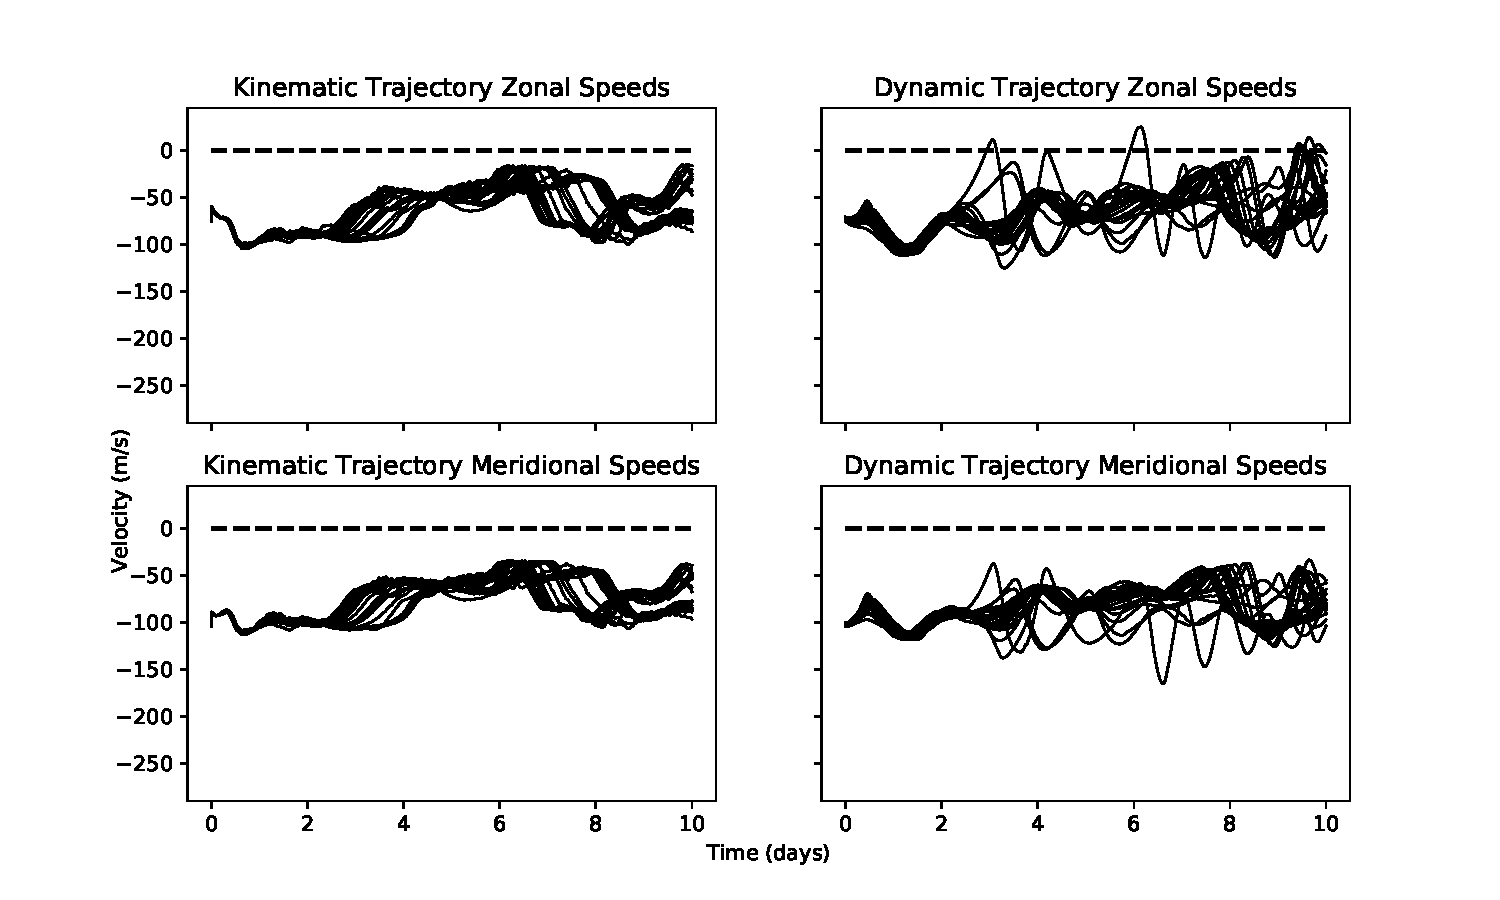
\includegraphics[width=\textwidth]{speed_subplots_180_negative.pdf}
    \centering
    \caption{For a timestep of 3 minutes, trajectory speed is compared to threshold speed.
    Solid lines represent the threshold speed minus the trajectory speed for a timestep of 3 minutes. 
    The dashed line at a velocity of zero represents the speed threshold.
    Note in the upper-right hand plot that the zonal speeds for some trajectories surpass the threshold. }
    \label{fig:speed_subplots_180_negative}
\end{figure}

\begin{figure}
    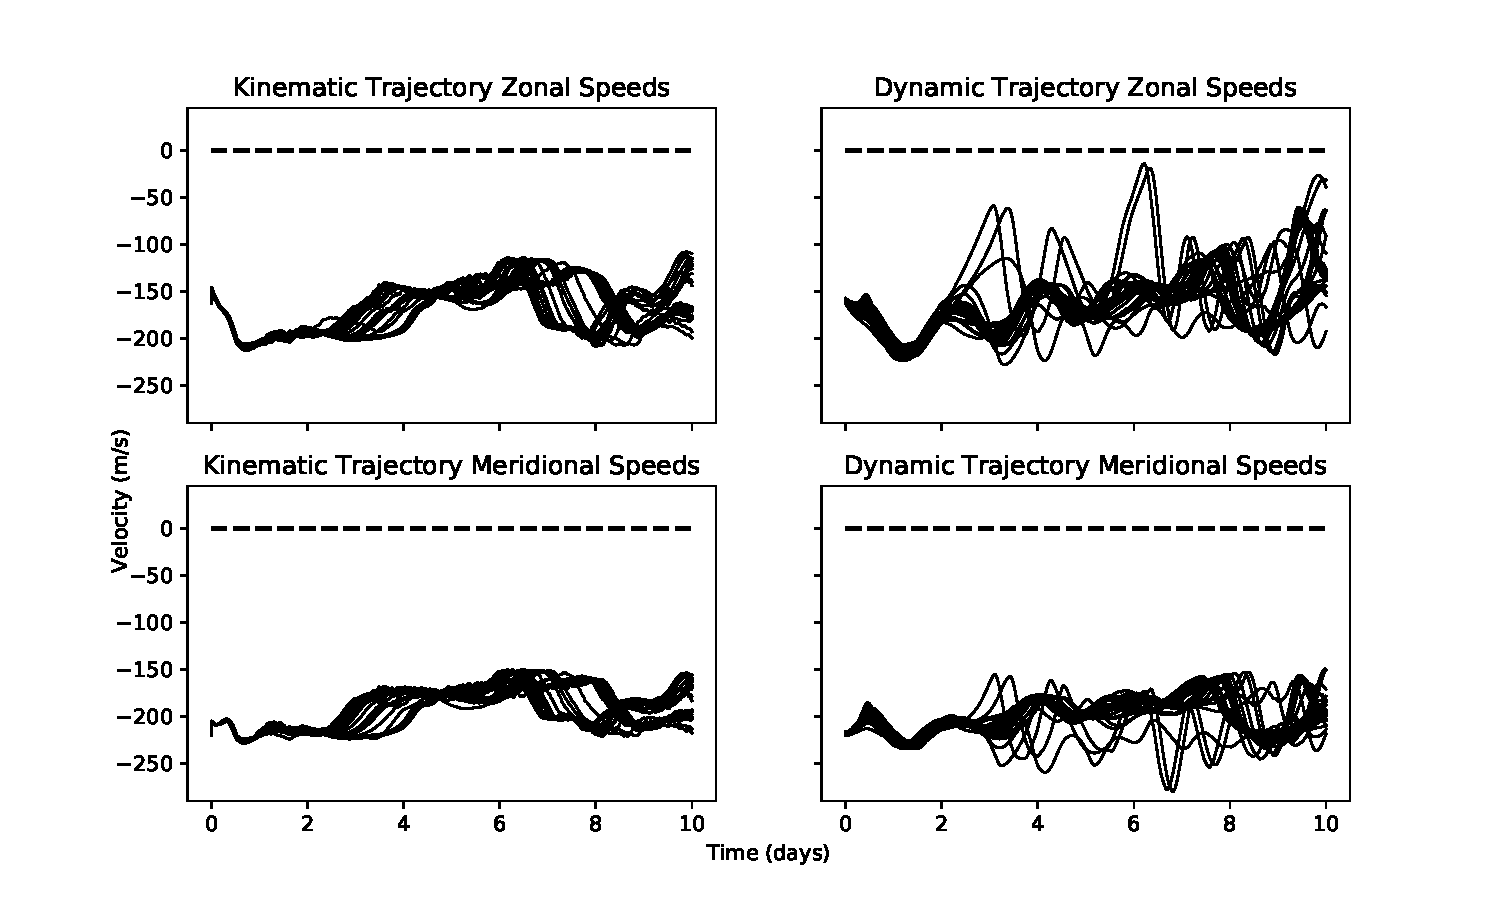
\includegraphics[width=\textwidth]{speed_subplots_90_negative.pdf}
    \centering
    \caption{For a timestep of 1 minute and 30 seconds, trajectory speed is compared to threshold speed.
    For this choice of timestep, all parcel velocities are below the threshold.}
    \label{fig:speed_subplots_90_negative}
\end{figure}

\section{Initializing velocity for the dynamic model}

The proposed method for determining initial trajectory velocity in the dynamic model was using the geostrophic wind, as expressed in Equations \ref{eq:u_g} and \ref{eq:v_g}.
The geostrophic wind is the theoretical wind calculating using the assumption that the Coriolis force balances the pressure gradient force.

This method is attractive for two reasons.
For one, it does not require additional data to be added to the dynamic model.
Geostrophic wind is calculated using the same grid of geopotential height gradients used for the advection equations \ref{eq:uvelocitygeo} and \ref{eq:vvelocitygeo}.
For another, initializing wind speed with geostrophic wind may reduce the inertial circle behavior observed in the dynamic model, which results from wind speeds deviating from the geostrophic approximation.

\begin{figure}
    \centering
    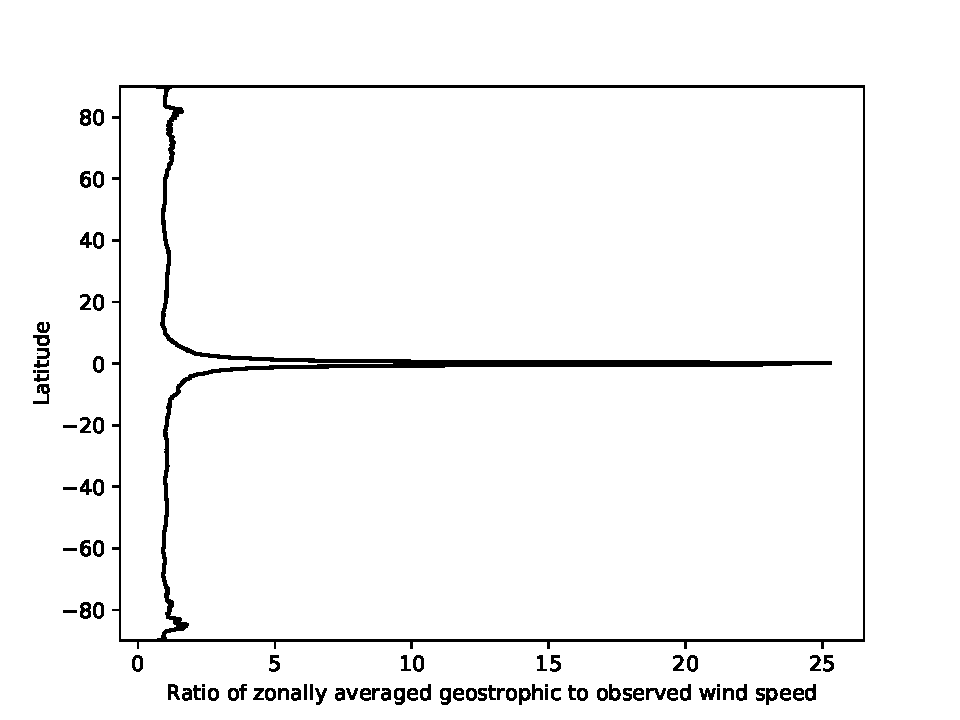
\includegraphics[width=\textwidth]{speed_ratio.pdf}
    \caption{The ratio of zonally averaged geostrophic wind speed to zonally averaged geostrophic wind speed as a function of latitude.
    Near the Equator, the ratio increases sharply, indicating that the geostrophic approximation is invalid there.}
    \label{fig:speed_ratio}
\end{figure}

However, the geostrophic approximation of wind speed breaks down near the equator.
Figure \ref{fig:speed_ratio} shows the ratio of zonally averaged geostrophic wind speeds to zonally averaged gridded wind speeds in the first file of the study period.
For most latitudes, the ratio is close to 1, which indicates that the geostrophic wind is a reasonable assumption.
Between 20S and 20N, the geostrophic wind becomes much greater than the observed wind. 
As the latitude goes to zero, the Coriolis parameter $f$ in Equations \ref{eq:uvelocitygeo} and \ref{eq:vvelocitygeo} blows up, and the resulting geostrophic wind becomes unphysical.

Since the dynamic model is intended to produce accurate trajectories for the whole Earth, the geostrophic wind cannot be used. 
Instead, velocities were initialized with the gridded wind values at the trajectory start locations. 
This may increase inertial circle prevalence, but the initial deviation from the geostrophic wind is damped by the dynamic model's friction term.
It also requires that wind speed data is available at every grid point in addition to geopotential height data, but this is likely to be the case when data from a forecast model like GFS is used.


